\documentclass{article}
\usepackage{float}
\usepackage{circuitikz}
\usepackage{cite}
\usepackage{amsmath,amssymb,amsfonts,amsthm}
\usepackage{algorithmic}
\usepackage{graphicx}
\usepackage{textcomp}
\usepackage{xcolor}
\usepackage{txfonts}
\usepackage{listings}
\usepackage{amsmath}
\usepackage{enumitem}
\usepackage{mathtools}
\usepackage{gensymb}
\usepackage{comment}
\usepackage[breaklinks=true]{hyperref}
\usepackage{tkz-euclide}
\usepackage{listings}
\usepackage{gvv}

%Enumering lower case roman numerals
%\renewcommand{\theenumi}{\roman{enumi}}
%\renewcommand{\labelenumi}{\theenumi)}

\newcommand{\mcomment}[1]{}

\begin{document}

\title{\textbf{Filter Design}}

\author{Soham Prabhakar More\\EE23BTECH11223}
\date{}

\maketitle
%-------------------------------------------------------------------------------
\section{Introduction}
We are supposed to design the equivalent FIR and IIR filter realizations for given filter number.
This is a bandpass filter whose specifications are available below.

\section{Filter Specifications}
\subsection{The Digital Filter}
\begin{enumerate}
\item {Passband:}
The passband is from \{4 + 0.6(j)\}kHz to \{4 + 0.6(j+2)\}kHz. \\
where
\begin{align}
    j=\brak{r-11000} \mod \sigma
\end{align}
where $\sigma$ is sum of digits of roll number and $r$ is roll number.\\
\begin{align}
    r &= 11223\\
    \sigma &= 9\\
    j &= 7
\end{align}
Hence, the un-normalized discrete time filter passband frequencies are $F_{p1} = 8.2$ kHz
and $F_{p2} = 9.4$ kHz. \\
The corresponding normalized digital filter passband frequencies are for sampling frequency $F_s = 48 kHz$:
\begin{align}
    \omega_{p1} &= 2\pi\frac{F_{p1}}{F_s} = 0.3417 \pi\\
    \omega_{p2} &= 2\pi\frac{F_{p2}}{F_s} = 0.3917 \pi
\end{align}

\item {Tolerances:} The passband ($\delta_1$) and stopband ($\delta_2$) tolerances are given to
be equal, so we let $\delta_1 = \delta_2 = \delta = 0.15$.

\item {Stopband:} The {transition band} for bandpass filters is $\Delta F = 0.3$ kHz on either side of the passband.

\begin{align}
    F_{s1} &= 8.2-0.3 = 7.9 \text{KHz}\\
    F_{s2} &= 9.4+0.3 = 9.7 \text{KHz}
\end{align}
\begin{align}
    \omega_{s1} &= 2\pi\frac{F_{s1}}{F_s} = 0.3292 \pi\\
    \omega_{s2} &= 2\pi\frac{F_{s2}}{F_s} = 0.4042 \pi\\
\end{align}
\end{enumerate}
\subsection{The Analog filter}
In the bilinear transform, the analog filter frequency ($\Omega$) is related to the corresponding digital filter frequency\brak{\omega} :
\begin{align}
  \Omega = \tan \frac{\omega}{2}
\end{align}
Using this relation, we obtain the analog passband and stopband frequencies as:
\begin{align}
    \Omega_{p1} &= 0.5949\\
    \Omega_{p2} &= 0.7067\\
    \Omega_{s1} &= 0.5687\\
    \Omega_{s2} &= 0.7366
\end{align}
respectively.
\section{The IIR Filter Design}
We are supposed to design filters whose stopband is monotonic and passband equiripple.
Hence, we use the Chebyschev approximation to design our bandpass IIR filter.
\subsection{The Analog Filter}
\begin{enumerate}

\item {Low Pass Filter Specifications:}  Let $H_{a, BP}(j\Omega)$ be the desired analog bandpass filter,  with the specifications provided in Section 2.2, and $H_{a,LP}(j\Omega_L)$ be the equivalent low pass filter, then
\begin{equation}
\Omega_L = \frac{\Omega^2 - \Omega_0^2}{B\Omega} \label{eq:freq_transform}
\end{equation}
where $\Omega_0 = \sqrt{\Omega_{p1}\Omega_{p2}} = 0.6484$ and $B = \Omega_{p2} - \Omega_{p1} = 0.1117$.

Substituting $\Omega_{s1}$ and $\Omega_{s2}$ in \eqref{eq:freq_transform} we obtain the stopband edges of lowpass filter
\begin{align}
    \Omega_{Ls1} &= \frac{\Omega_{s1}^2 - \Omega_0^2}{B\Omega_{s1}} = -1.527\\
    \Omega_{Ls2} &= \frac{\Omega_{s2}^2 - \Omega_0^2}{B\Omega_{s2}} = 1.483
\end{align}
And we choose the minimum of these two stopband edges
\begin{align}
    \Omega_{Ls} = \mbox{min}(\abs{ \Omega_{Ls_1}},\abs{ \Omega_{Ls_2}}) = 1.483.
\end{align}
\item {The Low Pass Chebyschev Filter Paramters:} The magnitude of frequency response of the low pass filter is given by
\begin{align}
    \abs{ H_{a,LP}(j\Omega_L)}^2 = \frac{1}{1 + \epsilon^2c_N^2(\Omega_L/\Omega_{Lp})} \label{eq:mag_freq_response}
\end{align}
The passband edge of the low pass filter is(by substituting passband edges in \eqref{eq:freq_transform}) $\Omega_{Lp}=1$.
Therfore ,
\begin{align}
    \abs{ H_{a,LP}(j\Omega_L)}^2 = \frac{1}{1 + \epsilon^2c_N^2(\Omega_L)} \label{eq:specification}
\end{align}
Where $c_N$ is the order $N$ chebyshev polynomial defined as:
\begin{align}
    c_N(x) &= \cosh(N \cosh^{-1}x)
\end{align}
or,
\begin{align}
    c_N(x) &= \cos(N \cos^{-1}x)
\end{align}
These polynomials can be calculated using the following recurrence relation:
\begin{align}
    c_{2N} &= 2c_{N}^2\brak{x} - 1\\
    c_{2N + 1} &= 2c_{N + 1}\brak{x}c_{N}\brak{x} - x\\
    c_{2N - 1} &= 2c_{N - 1}\brak{x}c_{N}\brak{x} - x \label{eq:cheby_poly_relation}
\end{align}
Imposing the band restrictions on \eqref{eq:mag_freq_response} \\
\begin{align}
    \abs{ H_{a,LP}(j\Omega_L)}^2 < \delta_2 \hspace{5pt}\text{for}\hspace{5pt} \Omega_L \geq \Omega_{Ls}\\
    1 - \delta_1 < \abs{H_{a,LP}(j\Omega_L)}^2 < 1 \hspace{5pt}\text{for}\hspace{5pt} 0 \leq \Omega_L \leq \Omega_{Lp}
\end{align}
we obtain:
\begin{eqnarray}
\label{lpdesign}
\frac{\sqrt{D_2}}{c_N(\Omega_{Ls})} \leq \epsilon \leq \sqrt{D_1}, \nonumber \\
N \geq \left\lceil \frac{\cosh^{-1}\sqrt{D_2/D_1}}{\cosh^{-1}\Omega_{Ls}} \right\rceil,
\end{eqnarray}
where $D_1 = \frac{1}{(1 - \delta)^2}-1$ and $D_2 = \frac{1}{\delta^2} - 1$ and $\left \lceil . \right \rceil$ is known as the ceiling operator .
\begin{table}[H]
    \centering
    
    \resizebox{0.4\textwidth}{!}{\begin{tabular}{|c|c|} % Define two centered columns with vertical lines
    \hline
    Parameter  & Value \\ % Row 1
    \hline
    $D_1$ & 0.3841 \\ % Row 2
    \hline
    $D_2$ & 43.444 \\ % Row 3
    \hline
    $N$ & 4 \\ % Row 4
    \hline
    $c_4\brak{x}$ & $8x^4 - 8x^2 + 1$\\
    \hline
    \end{tabular}}
    \caption{Parameter Table} % Table caption
    \label{tab:par_tab} % Table label for reference
\end{table}
we get $N\geq 4$ and $0.278 \leq \epsilon \leq 0.61$\\
The below code plots \eqref{eq:mag_freq_response} for different values of $\epsilon$ .
\begin{lstlisting}
https://github.com/Soham-More/EE1205/blob/main/filter_design/codes/epsilon.py
\end{lstlisting}
\begin{figure}[h!]
\centering
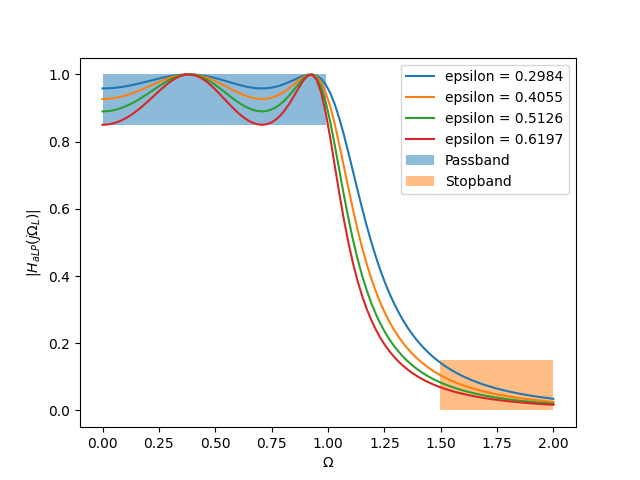
\includegraphics[width=1\columnwidth]{figs/epsilon_freq_res.png}
\caption{The Analog Low-Pass Frequency Response for $0.278  \leq \epsilon \leq 0.61$}
\label{fig:H_for_diff_eb}
\end{figure}

In \figref{fig:H_for_diff_eb} we can observe the equiripple behaviour in passband and monotonic behaviour in stopband. 
As the value of $\epsilon$ increases the value of $\abs{ H_{a,LP}(j\Omega_L)}$ decreases.\\

\item {The Low Pass Chebyschev Filter:} The next step in design is to find an expression for magnitude response in $s$ domain.

Using $s=j\Omega$ or in this case $s_{L}=j\Omega_{L}$ we obtain:
\begin{align}
    \abs{H_{a,LP}(j\Omega_L)}^2 = \frac{1}{1 + \epsilon^2c_N^2(\frac{s_L}{j})}
\end{align}
The poles are roots of the equation:
\begin{align}
    {1 + \epsilon^2c_N^2\brak{\frac{s_L}{j\Omega_{LP}}}} &=0\hspace{5pt}\text{where}\hspace{5pt} c_N(x) = cos\brak{Ncos^{-1}\brak{x}} \label{eq:pole_ques}
\end{align}
On solving \eqref{eq:pole_ques} we obtain poles :
\begin{align}
    s_{k} &= -\Omega_{Lp} \sin\brak{A_k}\sinh\brak{B_k} - j\Omega_{Lp}\cos\brak{A_k}\cosh\brak{B_k}
\end{align}
where $k$ is the index of the pole and \\
\begin{align}
    A_k &= \brak{2k+1}\frac{\pi}{2N}\\
    B_k &= \frac{1}{N} \sinh^{-1}\brak{\frac{1}{\epsilon}}
\end{align}

The below code computes the values of $s_k$ and stores it in a text file.
\begin{lstlisting}
https://github.com/Soham-More/EE1205/blob/main/filter_design/codes/analog_poles.c
\end{lstlisting}
The poles obtained are formulated in the table below.
\begin{table}[H]
    \centering
    
    \resizebox{0.51\textwidth}{!}{
    \begin{tabular}{|c|c|c|}
    \hline
    \textbf{$Pole$} & \textbf{$Value$} \\ \hline
    $s_1$ &-0.190705 - j1.032243 \\ \hline
    $s_2$ &-0.460404 - j0.427569 \\ \hline
    $s_3$ &-0.460404 + j0.427569  \\ \hline
    $s_4$ &-0.190705 + j1.032243 \\ \hline
    $s_5$ & 0.190705 - j1.032243\\ \hline
    $s_6$ & 0.460404 + j0.427569 \\ \hline
    $s_7$ & 0.460404 - j0.427569 \\ \hline
    $s_8$ & 0.190705 - j1.032243 \\ \hline
    \end{tabular}}
    \caption{Values of $s_k$}
    \label{tab:values poles sk}
\end{table}



The below code plots the pole-zero plot.
\begin{lstlisting}
    https://github.com/Soham-More/EE1205/blob/main/filter_design/codes/pole_zero.py
\end{lstlisting}
\begin{figure}[ht]
\centering
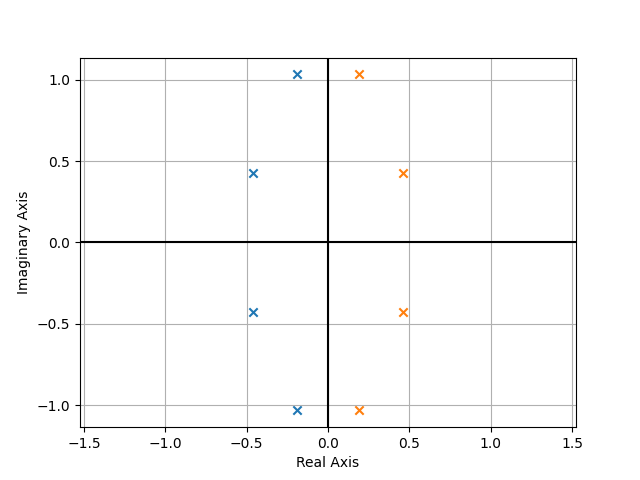
\includegraphics[width=1\columnwidth]{figs/polezero.png}
\caption{The Pole zero plot and all the poles lie on an ellipse. The left and right poles have been identified as shown.}
\label{fig:pole_zero_plt}
\end{figure}
The poles in the left half of the plane are considered in the design as we intend to design a stable system.\\
Therefore the magnitude response is written as :-
\begin{align}
    H_{a,LP}(s_L) &= \frac{G_{LP}}{\brak{s_L-s_5}\brak{s_L-s_6}\brak{s_L-s_7}\brak{s_L-s_8}}
\end{align}
where $G_{LP}$ is the gain of the Low pass filter. Refer to \tabref{tab:values poles sk} for $s_k$ values.\\

We know that from \eqref{eq:mag_freq_response}:-
\begin{align}
    \abs{ H_{a,LP}(s_L)} &= \frac{1}{\sqrt{1+\epsilon^2}} \text{at} \hspace{5pt} \Omega_{L}=1 \implies s_{L} = j \label{eq:Gain_eq_LP}
\end{align}
Substituting respective values in \eqref{eq:Gain_eq_LP} we get $G_{LP}=0.4166$
\begin{align}
     H_{a,LP}(s_L) &= \frac{0.4167}{\brak{s_L-s_5}\brak{s_L-s_6}\brak{s_L-s_7}\brak{s_L-s_8}}\\
     &= \frac{0.4167}{s_L^4 + 1.302218s_L^3 + 1.847886s_L^2 + 1.165209s_L + 0.435014}\label{eq:design}
\end{align}
\begin{figure}[ht]
\centering
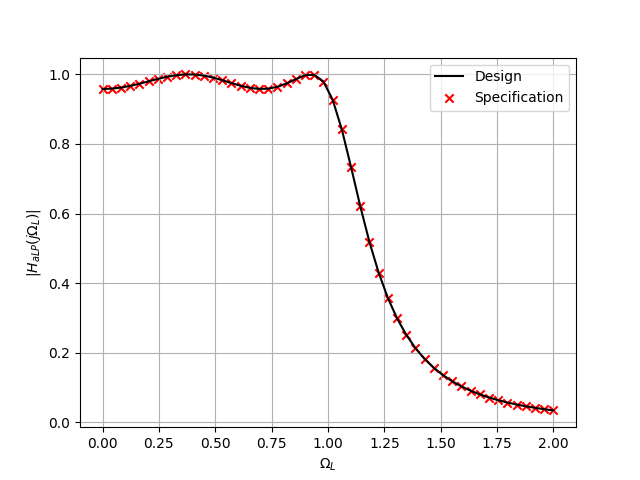
\includegraphics[width=1\columnwidth]{figs/spec.png}
\caption{Design vs Specification corresponding to \eqref{eq:design} and \eqref{eq:specification}}
\label{fig:design_vs_specf}
\end{figure}

\item {The Band Pass Chebyschev Filter:}
After verifying design with the required specifications the next step in design is to jump to required type of filter using frequency transformation.
\begin{align}
    s_L &= \frac{s^2 + \Omega_0^2}{Bs} \\
    H_{a,BP}(s) &= G_{BP}H_{a,LP}(s_L)\vert_{s_L = \frac{s^2 + \Omega_0^2}{Bs}},
\end{align}
As there is one to one correspondence between the filters so $\Omega=\Omega_{p1}$ should correspond to $\Omega_{Lp}$
\begin{align}
    s &= j\Omega_{p1}\\
    s_{L} &= \frac{(j\Omega_{p1})^2 + \Omega_0^2}{B(j\Omega_{p1})} \label{eq:res1} \\
    \abs{H_{a,BP}(j\Omega_{p1})} &= 1 \\
    G_{BP}\abs{H_{a,LP}(s_L)} &= 1 \label{eq:res2}
\end{align}
Substituting \eqref{eq:res1} in \eqref{eq:res2} we obtain Gain of required bass pass filter:
\begin{align}
    G_{BP} &= 1.0440
\end{align}
Thus the response in s domain
\begin{align}
    H_{a,BP}\brak{s} &= \frac{6.79\times 10^{-5}s^4}{s^8 + 0.146s^7 + 1.705s^6 + 0.185s^5 + 1.080s^4 + 0.078s^3 + 0.301s^2 + 0.011s + 0.031} \label{eq:magnitude_bandpass_sdom}
\end{align}
The expressions in the s-domain and gain factors are computed by writing a Python code. \\
In Figure 3, we plot $\abs{ H_{a,BP}(j\Omega)}$ as a function of $\Omega$ for both positve as
well as negative frequencies.  We find that the passband and stopband frequencies in the figure
match well with those obtained analytically through the bilinear transformation.
\begin{figure}[ht]
\centering
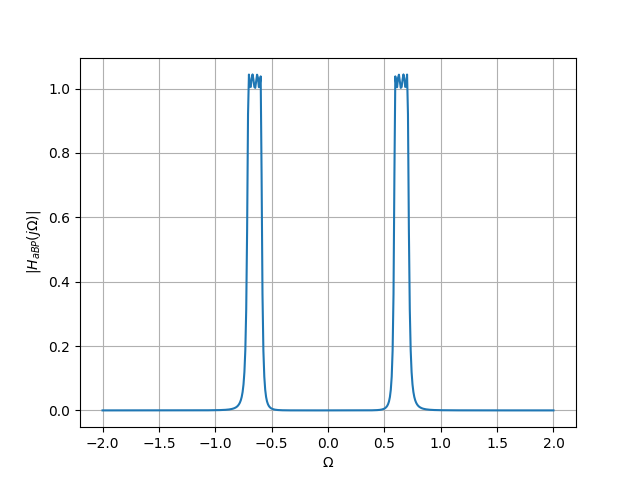
\includegraphics[width=1\columnwidth]{figs/H_BP.png}
\caption{The Analog Bandpass Magnitude Response from \eqref{eq:magnitude_bandpass_sdom}.The filter design specifications are satisfied}
\label{fig:band_pass_filter}
\end{figure}
\end{enumerate}

\subsection{The Digital Filter}
From the bilinear transformation, we obtain the digital bandpass filter from the corresponding analog filter as
\begin{align}
    H_{d,BP}(z) = GH_{a,BP}(s)\vert_{s = \frac{1-z^{-1}}{1 + z^{-1}}}
\end{align}
Substituting $s=\frac{1-z^{-1}}{1+z^{-1}}$ in \eqref{eq:magnitude_bandpass_sdom} and calculating expression using a python code we get :
\begin{align}
    H_{d,BP}(z) &= \frac{G\brak{1 - 4z^{-2} + 6z^{-4} - 4z^{-6} + z^{-8}}}{3.698 + -12.341z^{-1} + 30.916z^{-2} - 47.393z^{-3} + 58.606z^{-4} - 49.878z^{-5} + 34.243z^{-6} - 14.387z^{-7} + 4.537z^{-8}}
\end{align}

where $G=6.79\times 10^{-5}$
\begin{figure}[ht]
\centering
\includegraphics[width=1\columnwidth]{figs/Digital_BP.png}
\caption{Digital Specifications are met. Passband and stopband frequencies are same}
\label{fig:Digital_BPF}
\end{figure}

\section{The FIR Filter}
We design the FIR filter by first obtaining the (non-causal) lowpass equivalent using the Kaiser window
and then
converting it to a causal bandpass filter.
\subsection{The Equivalent Lowpass Filter}
The lowpass filter has a passband frequency $\omega_l$ and transition band $\Delta \omega = 2\pi \frac{\Delta F}{F_s} = 0.0125\pi$.
The stopband tolerance is $\delta=0.15$.The cutoff-frequency is given by :
\begin{align}
    \omega_{l} &= \frac{B}{2}\\
                &= 0.025\pi
\end{align}
\begin{figure}[h!]
\centering
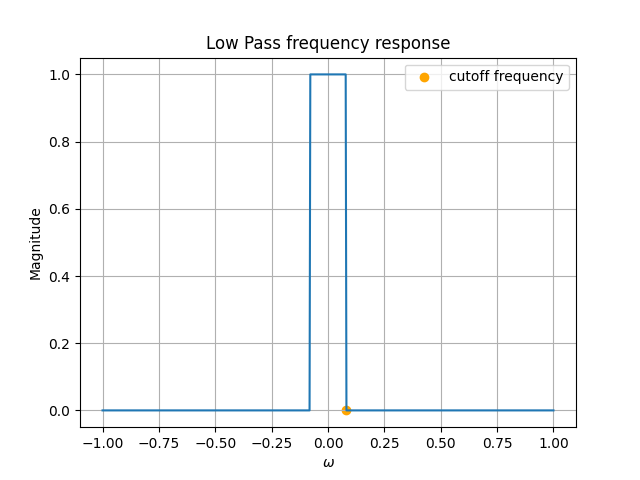
\includegraphics[width=1\columnwidth]{figs/FIR_ideal_w.png}
\caption{Frequency response of an ideal Low Pass Filter}
\label{fig:LPF_FIR_1}
\end{figure}
\begin{figure}[h!]
    \centering
    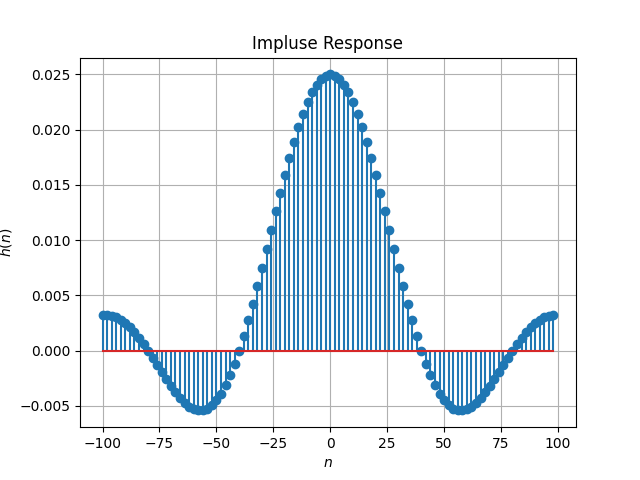
\includegraphics[width=1\columnwidth]{figs/FIR_ideal_n.png}
    \caption{Impulse response of an ideal Low Pass Filter}
    \label{fig:LPF_FIR_2}
\end{figure}

The impulse response of ideal Low Pass Filter is given by :
\begin{align}
    h\brak{n} =
\begin{cases}
    \frac{w_l}{\pi}, & \text{if } n = 0 \\
    \frac{\sin(w_l n)}{n\pi}, & \text{if} n \neq 0
\end{cases} \label{eq:h(n)_for_LPF}
\end{align}
From \eqref{eq:h(n)_for_LPF} we conclude that $h\brak{n}$ for an ideal Low Pass Filter is not causal and can neither be made causal by introducing a finite delay.
\subsection{The Kaiser Window}
Therefore we move on windowing the impulse response.A window function is chosen and multiplied. The Kaiser window is defined as
\begin{align}
    w(n) =
    \begin{cases}
    \frac{I_0\left[ \beta N \sqrt{1 - \left(\frac{n}{N}\right)^2} \right]}{I_0(\beta N)},
\indent -N \leq n \leq N, \indent \beta > 0 \nonumber \\
 0 \hspace{2.5 cm} \mbox{otherwise,}
 \end{cases}
\end{align}

\begin{enumerate}
\item  N is chosen according to
\begin{align}
    N \geq \frac{A-8}{4.57\Delta \omega},
\end{align}
where $A = -20\log_{10}\delta$.  Substituting the appropriate values from the design specifications, we obtain
$A = 16.4782$ and $N \geq 48$.


\item  $\beta$ is chosen according to

\begin{align}
    \beta N = \left\{ \begin{array}{ll} 0.1102(A-8.7) & A > 50 \\
0.5849(A-21)^{0.4}+ 0.07886(A-21) & 21 \leq A \leq 50 \\
0 & A < 21\end{array} \right.
\end{align}
The window function is defined as :
\begin{align}
    w\brak{n} =
\begin{cases}
    1, & \text{for } -48\leq n \leq 48 \\
    0, & \text{otherwise }
\end{cases} \label{eq:w(n)_for_Kaiser}
\end{align}
Therefore the desired impulse response is :
\begin{align}
    h_{lp} &= h_{n}w_{n}
\end{align}
\begin{align}
    h\brak{n} =
\begin{cases}
    \frac{\sin(w_l n)}{n\pi},  & \text{for } -48\leq n \leq 48 \\
    0 &\text{otherwise}
\end{cases} \label{eq:h(n)desired_for_LPF}
\end{align}
\end{enumerate}
\begin{figure}[h!]
\centering
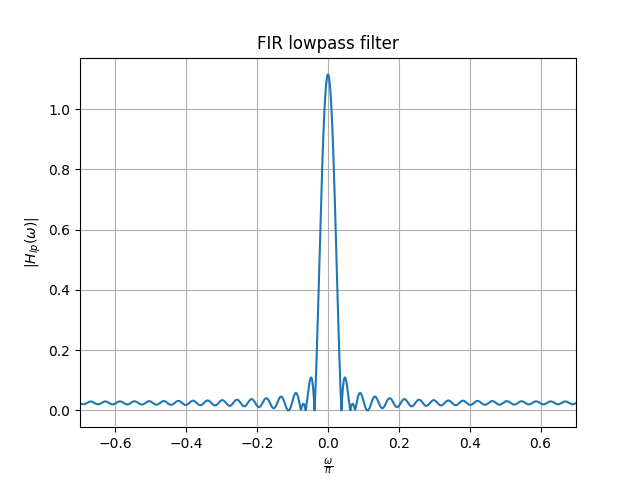
\includegraphics[width=1\columnwidth]{figs/FIR_kaiser_lp.png}
\caption{Magnitude Response of Low Pass Filter after using Kaiser Window}
\label{fig:Kaiser_LPF_response}
\end{figure}

\subsection{The Equivalent Band Pass Filter}
A Band-Pass Filter (BPF) can be obtained by subtracting the magnitude response of a Low-Pass Filter (LPF) with cutoff frequency $\omega_{p1}$ from another LPF magnitude response with cutoff frequency $\omega_{p2}$.

\begin{align}
    h_{BP}\brak{n} =
\begin{cases}
    \frac{\sin(w_{p2} n)}{n\pi} -\frac{\sin\brak{\omega_{p1}n}}{n\pi},  & \text{for } n\neq 0\\\
    \frac{\omega_{p2}-\omega_{p1}}{\pi} &\text{for} n= 0
\end{cases} \label{eq:h(n)desired_for_LPF}
\end{align}
\begin{align}
     \frac{\sin(\omega_{p2} n)}{n\pi} -\frac{\sin\brak{\omega_{p1}n}}{n\pi} &= 2\cos{\brak{\frac{\omega_{p2}n+\omega_{p1}n}{2}}}\sin{\brak{\frac{\omega_{p2}n-\omega_{p1}n}{2}}}\\
            &= \frac{2\cos{\brak{0.365n\pi}}\sin{\brak{0.025n\pi}}}{n\pi}
\end{align}
Multipying by window function we get :
\begin{align}
    h_{BP}\brak{n} =
\begin{cases}
   \frac{2\cos{\brak{0.365n\pi}}\sin{\brak{0.025n\pi}}}{n\pi},  & \text{for } -48\leq n \leq 48 \\
    0 &\text{otherwise}
\end{cases} \label{eq:h(n)desired_for_LPF}
\end{align}

\begin{figure}[h!]
\centering
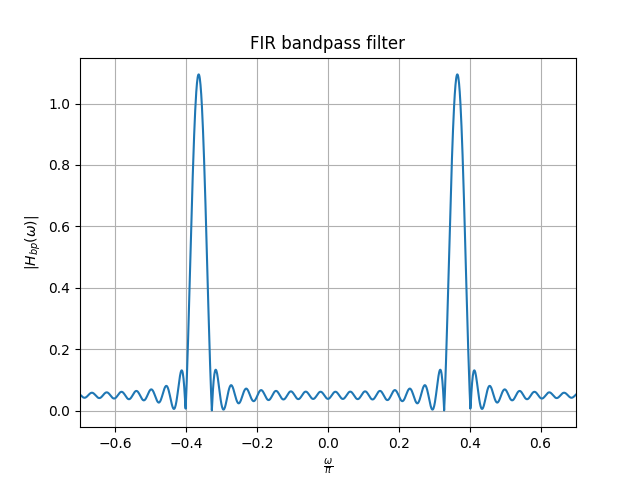
\includegraphics[width=1\columnwidth]{figs/FIR_kaiser_bp.png}
\caption{Magnitude Response of Band Pass Filter after using Kaiser Window}
\label{fig:Kaiser_BPF_response}
\end{figure}


\end{document}

